% 名城大学理工学部情報工学科卒業研究発表会
% ・名城大学理工学研究科情報工学専攻公聴会
% アブストラクトサンプル
% Last Update: 2021/11/13

\documentclass[a4paper, 9pt]{jarticle}
\usepackage{ieabst}
\usepackage{newenum}
\usepackage[dvipdfmx]{graphicx}

%タイトルが長い場合は,勝手に改行されます.
%% 「\\」の挿入で任意の位置に改行を入れられます.
\題目{ヒント数17の数独パズルの効率的な生成に関する研究}
\学籍番号{223426015}
\氏名{長尾 卓}
\研究室{山本}
% 旭研究室 宇佐見研究室 亀谷研究室 川澄研究室 小中研究室
% 佐川研究室 鈴木研究室 高比良研究室 田中研究室 寺本研究室
% 中野研究室 野崎研究室 坂野研究室 水沼研究室 向井研究室
% 柳田研究室 山田(啓)研究室 山田(宗)研究室 山本研究室
% 吉川研究室 米澤研究室


%1ページに入りきらない場合は,下の数字を少し小さめに変更.
\renewcommand{\baselinestretch}{1}

\begin{document}
\small

\twocolumn[\vspace*{29mm}] %タイトルが2行の場合は29mm→36mmに.
\begin{論文概要}           %この行は消してはいけません

\section{はじめに}
数独パズルは,ペンシルパズルの一種である.
ペンシルパズルとは,問題に対して答えを徐々に鉛筆で書き込んでいき,
答えを導くようなパズルのことである.
ペンシルパズルには,数独パズルのほかにスリザーリンクや虫食い算などが
知られている.数独パズルは,与えられたヒント
(例:\figurename{\ref{fig:problem_and_answer}}左)から,
1から9の数字を用いて縦,横,$3 \times 3$ブロックの
どの数字も重複させないように,マスを埋めていくパズルである.
\begin{figure}[b]
  \begin{minipage}[b]{0.49\linewidth}
    \centering
    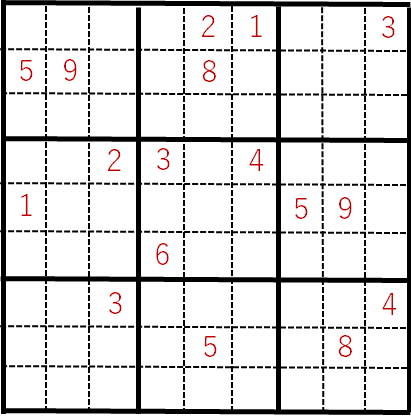
\includegraphics[width=3.5cm]{問題.png}
  \end{minipage}
  \begin{minipage}[b]{0.49\linewidth}
    \centering
    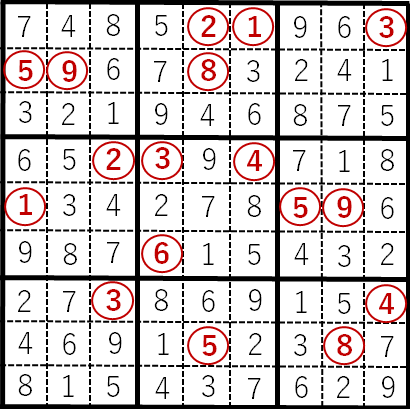
\includegraphics[width=3.5cm]{回答.png}
  \end{minipage}
  \caption{17個のヒントによる数独パズルの問題(左)とその解(右).}
  \label{fig:problem_and_answer}
\end{figure}
\figurename{\ref{fig:problem_and_answer}}左で与えられる問題の
答えは\figurename{\ref{fig:problem_and_answer}}右である.
また,1つの問題から得られる最終盤面はただ1通りである必要がある.
以降,数独パズルの最終盤面を「解」と表す.
先行研究 \cite{previous_research} では,ヒント数が少ない
数独パズルの問題を効率よく生成することを目的としていたが,
本研究では,ヒント数17の問題を効率よく生成することを目的とする.
ヒント数17の下限は17であることは \cite{seventeen_hints} により
証明されている.

\section{本研究の背景}
ヒント生成アルゴリズムは \cite{previous_research} の方法を
改善したものである.\cite{previous_research} のヒント生成アルゴリズムは,
まず,ヒント集合$H^{(0)} = \emptyset$を用意する.
$H^{(0)}$の右肩の数字はヒント集合のサイズを表す.
次に,適切なヒント$h$を$H^{(i)}$に添加していき,
$H^{(i)}$から得られる解の集合の大きさ$|S(H^{(i)})|$を徐々に減少させていく.
$h$はマスの位置$p$と数字$n$の組である.
適切な$h$とは,$H^{(i)}$に添加した後に最も$|S(H^{(i)})|$が減少するような
$h$のことである.
最終的には,$|S(H^{(i)})| = 1$となるまで$h$を$H^{(i)}$に添加して問題を生成する.
$h$の選択方法は,$H^{(i)}$から$S(H^{(i)})$を得て,得た解に出現した場所と
数字の組である複数の要素のうち最も出現回数が少ない要素を$h$とする.
なお,$H^{(i)}$から$S(H^{(i)})$を得るためには,
先行研究のようにバックトラック(BT)を用いればよい.
一方で,$H^{(i)} ~ (i < 14)$は十分に解集合の大きさが減少せず,
AXで解を列挙することは効率が悪い.
そのため,シミュレイテッド・アニーリング(SA)を用いることで
$H^{(i)}$から得られる解を偏りなく等確率に多く生成することを行い,
確率的に$h$を選択する.

\section{執筆要領}

\subsection{マージン}
マージンは以下を目安として,設定してください.

\begin{itemize}
\item 上マージン:30mm
\item 下マージン:27mm
\item 左マージン:25mm
\item 右マージン:25mm
\item カラム間マージン:7mm
\end{itemize}

\subsection{タイトル情報}
上部に以下のタイトル情報をページ全体にわたってセンタリングして1段組で記述してください.

\begin{itemize}
\item タイトル
\item 学籍番号と氏名
\item 所属研究室
\end{itemize}

\subsection{本文}
本文は2段組で記述してください.

本文は,必要に応じて節に分けて記述してください.
ただし,2 レベルまでとし,1, 1.1, 1.2, … のようにナンバリングしてください.

\subsection{図表}
図および表には,図1,表1のような通し番号と,名称を記述してください.ただし,図の場合には図の下部に,表の場合は表の上部に記述してください.

\subsection{参考文献}
参考文献は,本文内で\cite{paper1}\cite{paper2}のように引用し,本文に続いて,参照した文献のリストを掲載してください.参考文献は原則として以下のように記してください.

\begin{newenumerate}

\item {\bf 雑誌の場合}

著者: 標題, 雑誌名, 巻, 号, ページ (発行年).

\item {\bf 単行本の場合}

著者: 書名, ページ数, 発行所 (発行年).

\end{newenumerate}

\section{テンプレートおよびスタイルファイル}
Microsoft Word用のテンプレートと,\LaTeX 用のスタイルファイルを用意してあります.
招待を受けたGoogle Classroomからダウンロードして利用してください.

\subsection{Word用テンプレート}
マージンおよび以下のスタイルが登録してありますので,使ってください.
\begin{itemize}
\item アブストラクトタイトル
\item アブストラクト著者
\item アブストラクト所属
\item アブストラクト見出し1(1,2,3,...)
\item アブストラクト見出し2(1.1, 1.2, ...)
\item アブストラクト見出し3 ((1), (2),…)
\item アブストラクト本文
\item アブストラクト箇条書き(これ)
\item アブストラクト文献見出し(「参考文献」)
\item アブストラクト文献
\end{itemize}

\subsection{\LaTeX 用のスタイルファイル}
以下のように指定してください.

\begin{verbatim}
\documentclass[a4paper,9pt]{jarticle}
\usepackage{ieabst}
\usepackage{newenum}
\usepackage[dvipdfmx]{graphicx}
\end{verbatim}

newenum.styは,Wordテンプレートのスタイル「アブストラクト見出し3((1), (2),…)」に相当するものです.enumerate環境と同様に以下のように使用してください.
\begin{verbatim}
\begin{newenumerate}
\item {\bf アブストラクト見出し}
・・・
\end{newenumerate}
\end{verbatim}

その他は通常のコマンドを使って執筆してください.
そのほかの注意事項は,サンプルファイルを参照してください.

また,.latexmk ファイルを同梱したので,latexmk コマンド一発でコンパイルできます.

\section{PDFファイルについて}

Word,\LaTeX とも,PDFファイルを提出してください.
Wordの場合はdocxファイルを,\LaTeX
の場合はコンパイルに必要なソースファイル・図のファイルをまとめて圧縮したZIPファイル(特殊なスタイルファイルを用いた場合はそれも含める)を同時に提出してください.
WordファイルとPDFファイルについては圧縮する必要はありません.
PDFファイルの作成時は,フォントをすべて埋め込んでください.
また,アブストラクトを白黒プリンタで印刷する場合があり,その場合にカラー画像が見にくくなることを覚悟してください.


\section{\LaTeX 用サンプル}

\subsection{数式のサンプル}

数式のサンプルです.下記の式(\ref{eq:sample1})のように入力します.
\begin{equation}
\label{eq:sample1}
\left\{
\begin{array}{lcl}
\dot{\vec{x}}(t)&=&\vec{A}\vec{x}(t)+\vec{B}\vec{u}(t)\\
\vec{y}(t)&=&\vec{C}\vec{x}(t)
\end{array}
\right.
\end{equation}

\subsection{図表のサンプル}
図および表には,図\ref{fig:sample1},表\ref{tbl:sample1}のような通し番号と,名称を記述してください.ただし,図の場合には図の下部に,表の場合は表の上部に記述してください.

\begin{figure}[ht]
\centering
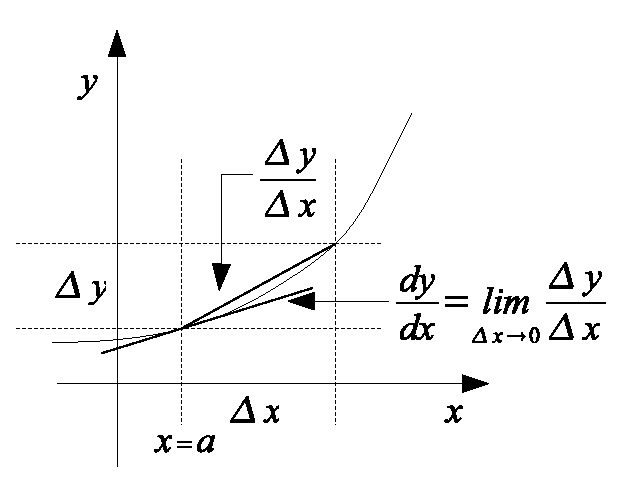
\includegraphics[width=0.9\columnwidth,clip]{2-1.eps}
\caption{EPS図のサンプル}
\label{fig:sample1}
\end{figure}

\begin{figure}[ht]
\centering
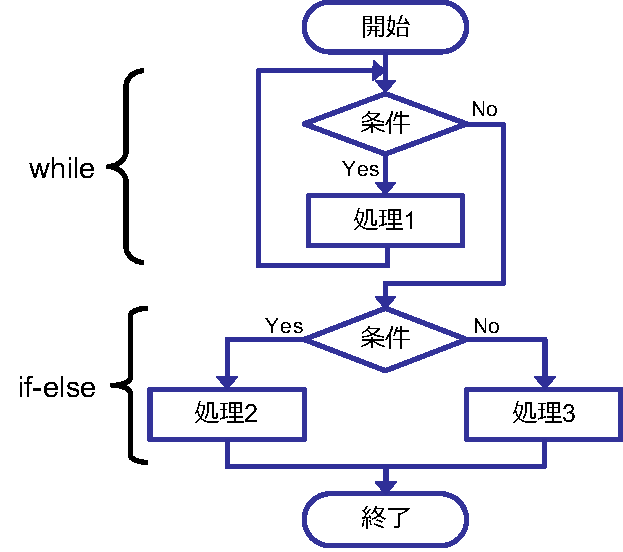
\includegraphics[scale=0.6,clip]{2-2.pdf}
\caption{PDF図のサンプル}
\label{fig:sample2}
\end{figure}

\begin{table}[ht]
\centering
\caption{表のサンプル}
\label{tbl:sample1}
\begin{tabular}{|c|c||c|c|} \hline
$p$ & $q$ & $p\rightarrow q$ & $(p\rightarrow q)\wedge q$ \\ \hline
T & T & T & T \\ \hline
T & F & F & F \\ \hline
F & T & T & T \\ \hline
F & F & T & F \\ \hline
\end{tabular}
\end{table}

\subsection{参考文献のサンプル}
参考文献引用のサンプルです~\cite{paper1}\cite{paper2}.


\begin{thebibliography}{10}

  \bibitem{previous_research}
  古川 湧:ヒントの少ない数独パズルの生成に関する研究.$2020$年度名城大学大学院理工学研究科修士論文(2021).
  
  \bibitem{nagao}
  長尾 卓:ビームサーチを用いたヒント数17の数独パズルの効率的な生成について.
  {\it ゲームプログラミングワークショップ2022論文集},pp. 96--103 (2022).
  
  \bibitem{seventeen_hints}
  G. McGuire, B. Tugemann, and G. Civario:
  There is no 16-clue Sudoku: Solving the Sudoku minimum number of clues problem via hitting set enumeration.
  {\it Experimental Mathematics}, 23:2, pp. 190--217 (2014).
  
  \bibitem{AX}
  D. E. Knuth: Dancing links. 
  {\it Millennial Perspectives in Computer Science}, pp. 187--214 (2000).

  % \bibitem{sa}
  % 池田 智悟,窪田 耕明:シミュレーテッドアニーリング概説.
  % \url{http://mikilab.doshisha.ac.jp/dia/monthly/monthly00/20000415/ikeuchi_kubota.pdf},参照2021-01-06 (2000).
  
  % \bibitem{beamsearch}
  % 長谷洋斗,川原純,笠原正治:解の多様性を考慮したビームサーチと局所探索法による
  % フロンティア法を高速化するための変数順序付け.
  % 第112回人工知能基本問題研究会,pp. 30--35 (2020).
  
\end{thebibliography}

\end{論文概要} %この行は消してはいけません
\end{document}
